\section{Introduction}

Benefiting from extensive training on large-scale corpora, large language models (LLMs) have demonstrated remarkable reasoning capabilities in solving complex problems~\citep{openai2024gpt4ocard, deepseekai2024deepseekv2strongeconomicalefficient, gemmateam2024gemma2improvingopen, qiu2025mindllm, zhao2023survey}.
One of the most impactful application areas is healthcare, which demands strong domain-specific knowledge and a high reliability standard~\citep{singhal2023large,thirunavukarasu2023large,nazi2024large}.
Previous studies have introduced benchmarks~\citep{yao2024medqa,jin2019pubmedqa,jiang2024mixtralexperts,wang2024mmlu} targeting different levels of medical reasoning tasks.

Despite their promising performance, the \textbf{readability} of LLM-generated responses, an essential factor for patient education, i.e., communicating health information to laypeople, has been largely overlooked and remains systematically underexplored.
\begin{figure}[htbp]
    \centering
    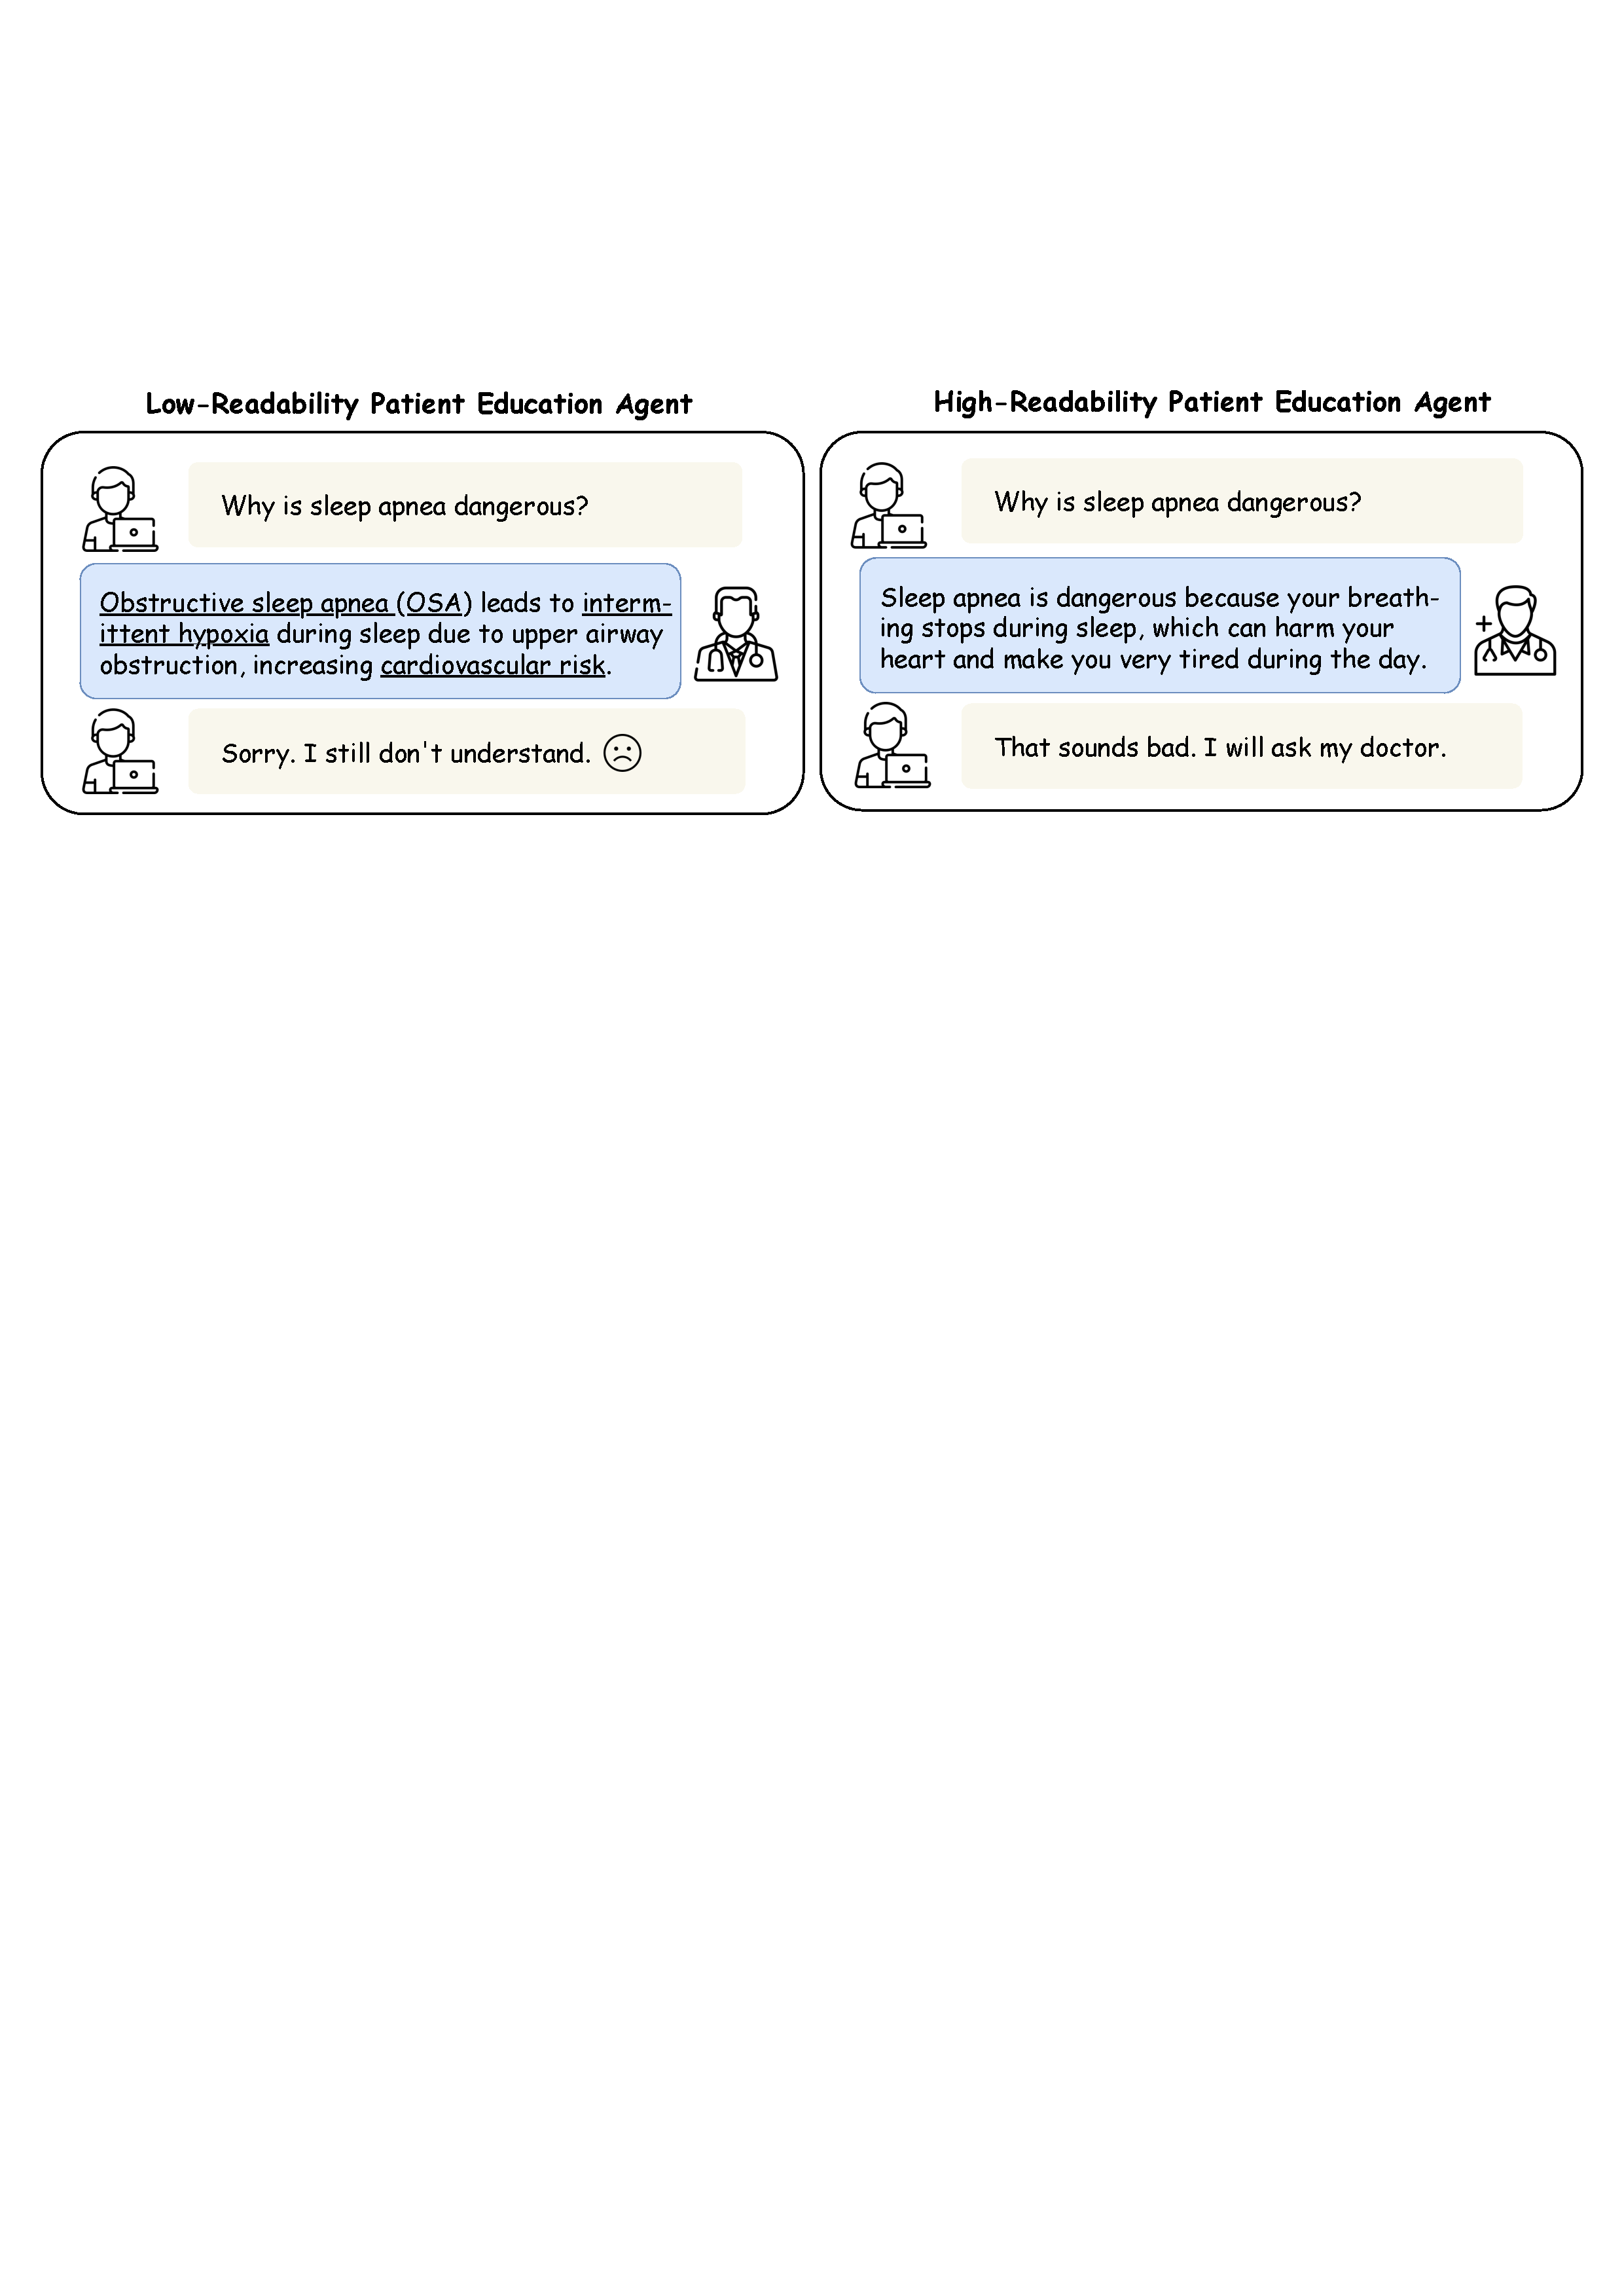
\includegraphics[width=1.0\textwidth]{figs/teaser_figv2.pdf}
    \caption{
        Two examples of user interactions with low- and high-readability public health agents. Medical jargon is underscored for the low-readability agent.
    }
    \label{fig:repqa-teaser}
\end{figure}

As shown in Figure~\ref{fig:repqa-teaser}, users without a medical professional background may find low-readability responses filled with medical jargon difficult to comprehend, whereas a plain-language answer can convey the same essential information more accessibly.
Moreover, state-of-the-art LLMs are increasingly optimized for complex reasoning~\citep{shao2024deepseekmath},
raising the question of whether these gains come at the expense of readability.
More advanced reasoning may lead to more technical responses that are harder for lay users to understand.

To evaluate the capabilities of LLMs in solving healthcare and medical problems, multiple benchmarks have been curated from diverse sources and presented in various formats~\citep{singhal2023large, lievin2024can, thirunavukarasu2023large}.
For instance, MedQA~\citep{jin2021disease}, MedMCQA~\citep{pal2022medmcqa}, MMLU~\citep{hendrycks2020measuring, wang2024mmlu}, and PubMedQA~\citep{jin2019pubmedqa} contain multiple-choice questions sourced from medical licensing examinations or PubMed articles, while LiveQA~\citep{abacha2017overview} and MedicationQA~\citep{abacha2019bridging} focus on long-form question answering for medicine-related problems.
Recent efforts have shifted toward more complex clinical tasks requiring multi-step reasoning and decision-making~\citep{yao2024medqa, chen2025benchmarking,nori2024medprompt,saab2024capabilities}, as well as incorporating additional modalities such as electronic health records~\citep{ou2025experience, bardhan2022drugehrqa, kweon2024ehrnoteqa}, radiology~\citep{zuo2025medxpertqa, liu2021slake}, and pathology~\citep{he2020pathvqa,lu2024multimodal}.
However, these benchmarks mainly evaluate the factual or reasoning accuracy of LLMs against professional examinations or specialized clinical tasks, rather than the readability of responses delivered to lay users.
% As summarized in Table~\ref{tab:dataset_comparison}, \repqa is the first to comprehensively evaluate the readability of LLM-generated responses to healthcare-related questions, using a dataset composed of publicly available medical queries from lay users.

\begin{table*}[t]
    \centering
    \caption{The comparison between \repqa and the existing healthcare benchmark datasets.}
    \resizebox{\textwidth}{!}{
    \begin{tabular}{ccccc}
    \toprule
    Dataset & Answer Format & Sources of Questions & Evaluation Metrics & Target Audience \\
    \midrule
    \midrule
    MedQA~\citep{jin2021disease} & Multiple Choice & Medical Examination & Accuracy & Medical Professionals \\
    MedMCQA~\citep{pal2022medmcqa} & Multiple Choice & Medical Examination & Accuracy & Medical Professionals \\
    MMLU~\citep{hendrycks2020measuring} & Multiple Choice & Medical Examination & Accuracy & Academic \\
    PubMedQA~\citep{jin2019pubmedqa} & Multiple Choice & PubMed Abstract & Accuracy & Clinical Researchers \\
    LiveQA~\citep{abacha2017overview} & Long Answer & National Library of Medicine & Human Evaluation & Consumers \\
    MedicationQA~\citep{abacha2019bridging} & Long Answer & MedlinePlus \& DailyMed & Human Evaluation & Medicine Consumers \\
    JAMA \& Medbullets~\citep{chen2025benchmarking} & Long Answer \& Multiple Choice & JAMA Challenge \& USMLE & NLG Metrics \& Accuracy & Medical Professionals \\
    \midrule
    \repqa & Long Answer & Public Health FAQs \& Experts & Readability \& Informativeness & Lay Users / Patients \\
    \bottomrule
    \end{tabular}
    }
    \label{tab:dataset_comparison}
\end{table*}

Beyond evaluation, a related line of research studies how to \emph{control} the complexity or reading level of text generated by LLMs.
Three main strategies have been explored:
(1) prompt- or instruction-based methods that modulate output difficulty by varying instructions or providing exemplars~\citep{tran2024readctrl, malik2024tarzan, barayan2024analysing, pu2023chatgpt};
(2) fine-tuning-based methods, e.g., \citet{chi2023learning} fine-tune language models on same-level paraphrasing datasets, and \citet{ribeiro-etal-2023-generating} employ PPO~\citep{schulman2017proximal} with the measured reading level~\citep{kincaid1975derivation} as a reward signal;
and (3) decoding-based methods that incorporate constraints during text generation~\citep{ribeiro-etal-2023-generating,luo2022readability}.
Several studies have further investigated the readability of LLM-generated responses regarding certain cancers~\citep{hershenhouse2024accuracy,gencer2024readability} or patient education handouts~\citep{swisher2024enhancing}.
While most prior work focuses on text summarization, \repqa specifically targets the readability of LLMs in patient education QA tasks.

In this study, a multidisciplinary team comprised of computer science, nursing, and public health experts introduced \textbf{\repqa} to conduct a comprehensive investigation into the \textbf{RE}adability of LLMs in \textbf{P}atient \textbf{E}ducation question-\textbf{A}nswering (QA) tasks.
A key strength of \repqa lies in its expert-grounded foundation: it comprises a high-quality test set with 533 QA pairs curated from 27 online public health resources.
% , all reviewed by professionals in nursing, public health, and clinical communication.
Different from prior related benchmarks (Table~\ref{tab:dataset_comparison}), \repqa focuses on frequently asked health questions from lay users or patients, and evaluates the readability of generated responses, an axis that prior healthcare benchmarks largely overlook, rather than only the underlying factual knowledge of the LLMs.
Additionally, we collected a large-scale corpus of 36,060 public health questions to serve as a post-training dataset, supporting the exploration of readability-enhancement strategies.

We evaluated 19 LLMs on \repqa using three readability metrics (Flesch-Kincaid grade level~\citep{kincaid1975derivation}, professional-language proportion, and Yngve depth~\citep{yngve1960model}) and an informativeness metric (the informative cosine between a response and its reference answer).
Our study targeted three capabilities: (i) answering at a specified reading level, (ii) inferring the appropriate level for a question, and (iii) using readability as a reward signal.
We found that current models mostly missed target levels and poorly identified appropriate levels, limiting their applicability for public-health agents.
We then benchmarked five existing readability-improvement strategies, including training-free controls (instruction-based prompting~\citep{ribeiro-etal-2023-generating,malik2024tarzan}, CoT~\citep{wei2022chain}, and lookahead decoding~\citep{ribeiro-etal-2023-generating}) and reinforcement-learning fine-tuning (GRPO~\citep{shao2024deepseekmath} and DAPO~\citep{yu2025dapo}).
Readability-aware post-training yielded large gains in readability metrics but could reduce the informativeness of responses due to over-simplification, underscoring a difficult readability–informativeness trade-off.
This study will offer insights for future work on developing trustworthy healthcare agents and educational domains~\citep{wang2024large}.
In summary, our contributions are listed as follows:
\begin{itemize}[leftmargin=*]
\item We introduced \repqa, an expert-crafted benchmark for patient education QA aimed at lay users, with three readability metrics (Flesch–Kincaid grade, professional-language proportion, and Yngve depth), an informativeness metric (the informative cosine between a response and its reference answer), and a large-scale (36,060) expert-reviewed public health questions for post-training.

\item We conducted a study on 19 LLMs, revealing that most models failed to (i) generate at requested reading levels and (ii) identify an appropriate level for a given question.

\item We benchmarked a range of existing strategies for improving LLM readability, spanning training-free control (prompting, chain-of-thought, and lookahead decoding) and reinforcement-learning fine-tuning (GRPO and DAPO). Readability improved substantially, but often at the expense of informativeness, highlighting a challenging readability–informativeness trade-off.
\end{itemize}
